\section{Durchführung}
\label{sec:Durchführung}
\subsection{Versuchsaufbau}
Der Aufbau ist in der Grafik \ref{fig:Aufbau} abgebildet.
\begin{figure}[H]
\center
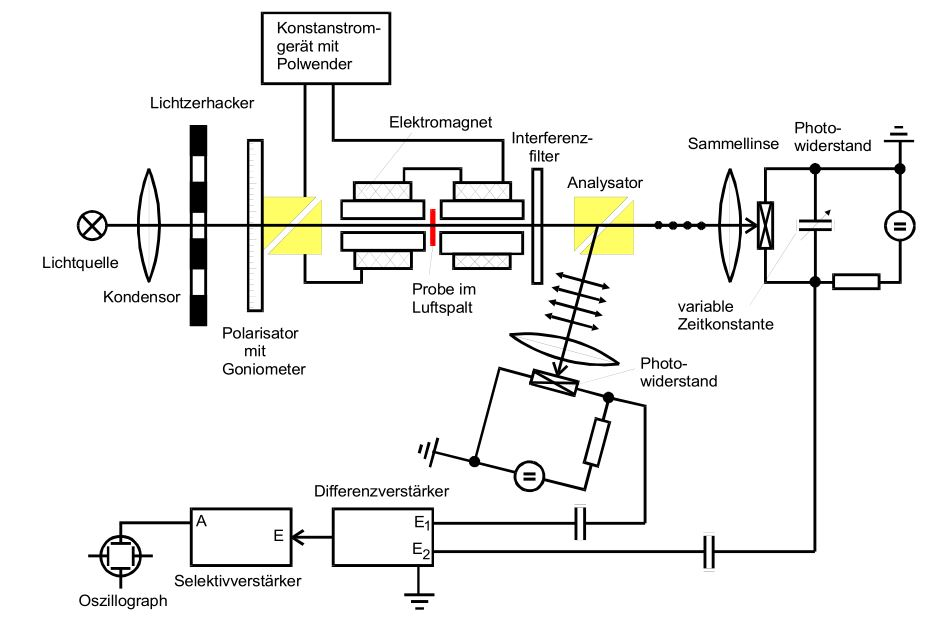
\includegraphics[width=0.8\textwidth]{pics/Aufbau.jpg}
\caption{Schematische Darstellung des Versuchsaufbaus \cite{Anleitung}.}  %?? ändern
\label{fig:Aufbau}
\end{figure}
Als Lichtquelle wird eine Halogen-Lampe mit überwiegend im Infrarot liegendem Emissionsspektrum verwendet.
Durch eine Linse wird der Lichtstrahl gebündelt.
Anschließend zerteilt ein Lichtzerhacker das einfallende Licht in Impulse um ein möglichst scharfes Signal messen zu können, indem
ein Großteil des Rauschen durch einen auf die Frequenz der Impulse eingestellten Verstärker rausgefiltert werden.
Ein Glan-Thompson Prisma dient als Polarisator. Es spaltet den einfallenden Lichtstrahl in zwei
unterschiedliche senkrecht auf einander polarisierte Strahlen. In einem Elektromagneten trifft der Lichtstrahl auf die Probe und anschließend auf einen
Interferenzfilter, mit dem eine bestimmte Wellenlänge $\lambda$ herausgefiltert wird.
Im Analysatorprisma wird der Lichtstrahl geteilt und auf zwei Photowiderstände
geleitet. Die beiden Signale werden an einen Differenzverstärker weitergegeben,
welcher die Differenz der zwei Spannungen bildet. Die entstehende Impuls wird zu einem Selektivverstärker geleitet,
welcher auf die Frequenz des Lichtzerhackers abgestimmt ist.
Das Signal kann am angeschlossenen Oszillograph abgelesen werden.
\subsection{Messprogramm}
Nach der Justierung des Versuchsaufbaus werden drei Proben vermessen. Einmal ein undotiertes
Galliumarsenid (GaAs) und zwei verschieden n-dotierte GaAs-Proben. Die Proben werden mit jeweils
acht verschiedenen Interferenzfiltern vermessen.\\
Hierzu wird am Goniometer der Winkel des Prismas so eingestellt bis die Differnzintensität annähernd
verschwindet. Dieses Vorgehen wird nun mit eingeschaltetem Elektromagneten wiederholt.
Die beiden Winkel werden notiert und über die Differenz $\theta=\theta_1-\theta_2$ lässt sich der Faradaywinkel bestimmen.\\
Abschießend wird die Probe entfernt und das Magnetfeld mit einer Hallsonde vermessen, um  
die magnetische Feldstärke am Ort der Probe zu ermitteln.
